\chapter{Discussion}

This project took a protein-first approach to the discovery of structured RNAs, with a focus on \ac{RNP} complexes.
A discovery pipeline, taking a protein domain probabilistic model and bacterial genome space, was developed and then applied to the search for an RNA light switch anchored by the \ac{BLUF} domain.
Further, a novel approach to the clustering of RNA elements was developed.

\section{Discovery pipeline}

The bioinformatic discovery pipeline was the core of this project, and was developed to identify novel structured RNA elements anchored by protein domains.
It was tested with a positive control, the \ac{FMN}-riboswitch-associated RibD C-terminal domain and a negative control set of membrane-associated protein domains.
Anchoring the discovery pipeline with the \ac{BLUF} domain then identified a set of candidate structured RNA elements.

\subsection{Bioinformatic approach to RNA discovery}

The bioinformatic approach to RNA dicovery taken in this project utilised many existing tools and methods, and combined them into a novel pipeline, as well as developing a novel approach to clustering RNA elements.
Key tools used in the discovery pipeline were MMseqs2 \citep{Kallenborn2025} for sequence homology search and R-scape \citep{Rivas2017} for covariation analysis.
Overall the bioinformatic approach was successful in identifying the \ac{FMN} riboswitch from the RibD C-terminal domain, and in identifying a set of candidate structured RNA elements associated with the \ac{BLUF} domain.

A variety of other bioinformatic tools were used in this project with varying levels of success and reliability, and many of them were not presented in the results or methods.
CMfinder v.0.4.1.18 \citep{Yao2006} was tested as a candidate method for identifying structured RNA elements, but was found to be unsuitable for this project.
It was found to be computationally expensive and to crash on large datasets, such as the \ac{FMN} riboswitch positive control dataset with 880 sequences, with uninformative error messages.
CMfinder has been used successfully by \citet{Geissler2026} across 202 genomes, and other studies \citep{Roth2014, Sack2025, Weinberg2015}, perhaps due to a smaller dataset sizes, or different computational resources.
The CMfinder software was also found to be difficult to install and run, with dependencies that were not well documented.

Additionally, CMCompare \citep{Eggenhofer2013} was tested as a candidate method for clustering covariance models.
It was found to no longer be maintained, and the software was not compatible with the current version of Infernal.
Web-based CMCompare was also no longer available.
Some work went into trying to get the software to run, but it was ultimately unsuccessful.

\subsection{Positive control}

A positive control preparation pipeline was developed to generate a set of positive control sequences for the discovery pipeline.
This also provided evidence that modern bioinformatic tools are capable of identifying biologically relevant \ac{RNP} systems and cis-regulatory elements and protein relationships, from the RNA direction.
It was found that the \ac{FMN} riboswitch is associated with the RibD C-terminal domain, which is a protein domain that is involved in the biosynthesis of riboflavin, and is coded on the rib operon downstream of the riboswitch \citep{Mironov2002}.
The \ac{SAM} riboswitch was found to be associated with a Cys/Met metabolism PLP-dependent enzyme domain, which matches the \emph{metB} gene (Pfam \citep{Paysan-Fafosse2025}) found by \citet{Tang2020} to be under the control of the \ac{SAM} riboswitch.
Additionally, the Fluoride riboswitch was found to be associated with a CrcB-like protein camphor resistance domain, which is consistent with the known biology of the fluoride riboswitch \citep{Baker2012}.
These riboswitch examples illustrate the ability to rediscover known riboswitch protein systems begining with a known RNA element, and provided a set of potential positive control pairs for the discovery pipeline.

The \ac{CRISPR}-DR42 RNA family was used to demonstrate this protein:RNA pair discovery in the context of a known \ac{RNP} system.
The \ac{CRISPR}-DR42 RNA family was found to be associated with the CRISPR-associated protein Cas2 domain.
Cas1 and Cas2 form a complex which binds to \ac{CRISPR} repeat sequences (like \ac{CRISPR}-DR42) \citep{Barrangou2007}.
This illustrates the ability to rediscover a known \ac{RNP} system from the RNA direction.
Unfortunately the discovery pipeline is currently not set up to extract the intergenic regions of the opposite strand to the identified coding sequence and the \ac{CRISPR}-DR42 RNA family was found to be located primarily on the opposite DNA strand to the Cas2 coding sequence (Table \ref{tab:results_summary}).

A single positive control was used: the \ac{FMN}-riboswitch-associated RibD C-terminal domain, which was chosen for its clear biological association with a protein and its relative conservation across a wide set of bacterial species.
A larger set of positive control pairs would better validate the discovery pipeline, and should be considered for future work.

The discovery pipeline, run using a RibD C-terminal domain anchor, yielded a set of candidate RNA elements with strong similarity to the \ac{FMN} riboswitch (Figure \ref{fig:drh-top-structures}, Figure \ref{fig:candidate-clustering}).
This shows, first, that for the \ac{FMN} riboswitch the intergenic sequences neighbouring a protein domain anchor contain enough information to identify a structured RNA element.
Secondly, it suggests that the discovery pipeline can recover this structured RNA element, although sensitivity was not formally quantified.
Overall, this provides proof of principle that a protein-first approach to RNA discovery is feasible.
This rests on a single, relatively easy positive control, however: the \ac{FMN} riboswitch is highly conserved and well characterised, and the protein domain profile used as the anchor was generated from sequences neighbouring the Rfam-annotated riboswitch.
Recovery of this signal is therefore a best-case scenario, and does not show that the pipeline will detect less conserved or more divergent structured RNAs.
Additionally it does not test an RNA protein complex, which is one of the goals of this project.

\subsection{Negative control}

There are many difficulties in the curation of a negative control set for a discovery pipeline stemming from the difficulty of proving a negative.
It is impossible to prove that a given protein domain is not associated with a structured RNA element, and so it is difficult to curate a negative control set for the discovery pipeline.
The negative control sshould represent the background conservation and random covariance of nucleotide pairs by chance neighbouring conserved protein coding genes.
These criteria ruled out randomly generated sequences, or shuffled sequences.
Beyond being biologically unrealistic, the covariance analysis tool, R-scape, already tests against a null model of covariation due to phylogeny but independent of structure \citep{Rivas2017}.

As an imperfect solution, a set of membrane-associated protein domains was curated as negative control anchors.
The main rationale being that structured RNA elements are rare across genomes \citep{Geissler2026,Weinberg2015}, and so it is unlikely that a random set of protein domains would be associated with structured RNA elements.
These were the SecY domain, a protein translocase subunit, YgaP-like domain, a transmembrane protein domain, the YadA-like domain, an outer membrane protein C-terminal domain, and the Flagellin N-terminal domain.

Of the four negative control domains, the YadA-like domain returned no candidates with a significant covarying pair, the SecY and YgaP-like domains returned a few weak candidates (one to two covarying pairs, F-measures of 4.44 to 6.06), and the flagellin domain returned nine candidates.
Eight of the flagellin candidates were similarly weak (one to four covarying pairs, F-measures of 1.20 to 8.00), which gives an empirical baseline for the covariation signal expected when no known structured RNA is present.
The ninth, candidate 327, had 11 covarying pairs and an F-measure of 43.14, within the range of the \ac{FMN} riboswitch candidates.
However, a BLASTX search matched this candidate to pseudaminic acid synthase, so its signal most likely reflects conservation of a protein-coding sequence rather than a structured RNA.
The match was in reading frame $-1$, indicating that the coding sequence is on the opposite strand to the flagellin anchor gene, within the flanking region examined by the discovery pipeline.

This outcome is informative rather than a failure of the control.
It shows that conserved protein-coding sequence in the flanking regions can generate a strong covariation signal that the covariance analysis alone does not rule out, so the BLASTX check for coding sequence (Section~\ref{subsec:rfam-blastx-check}) is a necessary step before a candidate is interpreted as a structured RNA.
Alternatively the discovery pipeline could define intergenic regions as the non-coding sequence between two coding sequences, regardless of strand.
This was the original implementation but was changed to be more permissive.

The flagellin domain is also a less certain negative control than the other three domains.
RNA-based regulation of flagellar gene expression has precedent in the literature, for example small RNAs that regulate the flagellar regulator FlgM in enteric bacteria \citep{Mika2013}.
A conserved structured RNA near a flagellin gene is therefore not implausible, and the weak flagellin candidates are best treated as background of uncertain status rather than as confirmed false positives.
The baseline ranges given above include them; excluding flagellin entirely, the SecY and YgaP-like candidates had F-measures of 4.44 to 6.06 and one to two covarying pairs.
Finally, this places the \ac{BLUF} candidates in context: their F-measures (11.27 and 5.00) and numbers of covarying pairs (4 and 2) are close to, or within, the range of the other negative control candidates, so their covariation signal is not by itself convincing evidence of a structured RNA.

\subsection{Searching with \ac{BLUF}}

\ac{BLUF} was chosen as a proof-of-concept search target for its potential to be involved in an \ac{RNP} 'light switch' complex.
Two candidates were identified, with weak covariation signal (F-measures of 11.27 and 5.00, and 4 and 2 covarying pairs).
Convincing evidence of covariation would be a higher F-measure and covarying pairs with higher statistical power (these were 0.07 for all candidate 130 pairs, and 0.07 and 0.24 for the candidate 332 pairs).
AlphaFold 3 interaction predictions were made for the two candidates with the \ac{BLUF} domain, and the results were compared to a negative control (BLUF with a random RNA).
Convincing evidence of a specific interaction between the candidates and the \ac{BLUF} domain would be an \ac{ipTM} score above 0.6, which is the threshold for a confident prediction according to AlphaFold 3 guide documentation \citep{Embl-Ebi2026}.

It is also unknown whether these structures, if they exist, are biologically relevant, or what function they might have.
Beyond this, they may not interact with the \ac{BLUF} protein domain at all, and may instead be involved in other biological processes, including acting as cis-regulatory elements.
The RNA elements may also be functioning with other neighbouring protein domains, and may simply have been picked up through conservation of coding sequence order and proximity to the \ac{BLUF} domain.
\citet{Tamames2001} described the conservation of gene order in prokaryotic genomes, noting high conservation in closely related prokaryotic species.
This could be tested with the existing positive control preparation pipeline and a set of representative genomes from a range of prokaryotic species in future work.
This approach could indicate if other protein domains are conserved in the neighbouring coding sequences of any other identified homologs of the new candidate RNAs.

\section{Covariance model clustering approach}

\subsection{Developing a novel approach to covariance model comparison} % I need to come up with a better heading

There is a gap in bioinformatic tools for a fast, working, reliable and statistically defensible similarity scoring for covariance models, the predictive models describing the structure and sequence of conserved RNA elements.
The inspiration for covariance model clustering came from a lack of tools to quantitatively compare the positive control candidates to the Rfam annotated \ac{FMN} riboswitch consensus model.
There are clear applications of this approach beyond validating the positive control candidates of this project, including identifying relationships between RNA families for database curations.

Preliminary benchmark testing of the developed approaches was done with a curated set of 44 Rfam families from various clans, and the results of pairwise comparisons were compared to the annotated clan relationships \citep{Ontiveros-Palacios2025}.
Clans are curated groups of RNA families from Rfam that are believed to be evolutionarily related, and so are assumed to be more homologous to each other than to other families.
This was an imperfect test, as there is no ground truth for the evolutionary relationships of RNA families, and so the annotated clans are only a proxy for homology.
For example, many Rfam micro RNA families are not annotated as belonging to a clan, but share similar hairpin structures \citep{Xue2005}.
This structural similarity was detected by all of the following approaches.

The \% coordinate overlap identity reported in the results is a simple measure of how similar the seed sequences of two covariance models are over a small sequence space.
It does not take into account the structure or probabilistic nature of the covariance models.
The variable size of the seed aligned sequence set also makes this measure unreliable, as a small seed set will have a higher chance of overlap by chance than a large seed set.

The CMCompare tool \citep{Eggenhofer2013}, although not useable as described earlier, goes about comparing models in an interesting way.
It uses the models themselves to calculate a sequence which is likely to be homologous to both models, and then uses the bitscore of that sequence against each model as a measure of similarity.
This takes advantage of the evolutionary assumption that a common ancestor of two related RNA elements can be found and that the distance to these is a measure of similarity.
Rather than reimplementing CMCompare, a genetic algorithm was developed to estimate a sequence that is likely to be homologous to both models, and then use the bitscore of that sequence against each model (a measure of the probability a sequence belongs to a particular model) as a measure of similarity.
This approach was found to reliably rediscover clan relationships in the Rfam database.
It however lacks an obvious null model to test against, and so the statistical significance of the similarity score is difficult to interpret.

Covariance models can be used to emit a distribution of sequences that are likely to be homologous to the model.
Given two covariance models, the overlap of their emitted sequence distributions can be used to measure their similarity.
This overlap can conveniently be measured by the models themselves, which can calculate bitscore likelihoods that the emmitted sequences are homologous to the other model.
This overlap thought led to the development of the median score and score distribution pairwise scoring approaches.
The two approaches diverge in how they measure the overlap of the two distributions and in how they test against a null model of overlap by chance.

The median score approach measures the overlap of the two distributions by taking the median of the bitscore likelihoods of the emmitted sequences from one model against the other model.
Medians were used as opposed to means becuase of the observed skewed distribution of the bitscores (Figure~\ref{fig:ks-worked-example}).
This approach fortunately has a reasonably obvious null model: the median of populations of dinucleotide shuffled emitted sequences from one model against the other model.
Dinucleotide shuffling preserves the dinucleotide frequencies of the original sequences, and so preserves the overall sequence composition and length \citep{Altschul1985}.
This null therefore acts to test against length and compositional bias of the models, and against the possibility of overlap by chance.
It also leads to a simple and intuitive empirical p-value, which is the proportion of shuffled medians that are greater than or equal to the observed median.
This approach was found to be effective at clustering Rfam RNA families into their annotated clans.
This approach involved searching many null sequeces against the models which was computationally expensive when compared to the optimal sequence approach.

Also observeable from the distribution of bitscores is that the distributions of related models, although not always particularly right shifted, are often flatter and wider than the distributions of unrelated models and to shiffled sequence distributions (Figure~\ref{fig:ks-worked-example}).
This led to the development of the \ac{KS} D statistic approach, which measures the overlap of the two distributions by comparing their cumulative distribution functions against the null shuffled sequence distributions \citep{Smirnov1939}.
This has the advantage of being computationally cheaper than the median score approach, as it does not require searching as many null sequences against the models.
This approach was also found to be effective at clustering Rfam RNA families into their annotated clans, and was used to cluster the positive control candidates with the \ac{FMN} riboswitch.

\subsection{Applications to iterative combination of covariance models}

One application for this clustering approach is to integrate it into a discovery pipeline to identify similar covariance models and merge them to create a new model that captures the shared features of the original models.
As could be seen in the positive control candidates, some of the candidates are likely to be homologous to each other, but are not similar enough to be detected by classical homology search methods.
If a new model could be created from these candidates, it could be used to identify more distant homologs and improve the sensitivity of RNA discovery pipelines, and power of any covariance analysis.
Figure \ref{fig:cluster-merging} illustrates this idea, showing three structured RNA elements that have been identified by local alignment, which are homologous to each other, but are not similar enough to be detected by classical homology search methods.

\begin{figure}[H]
    \centering
    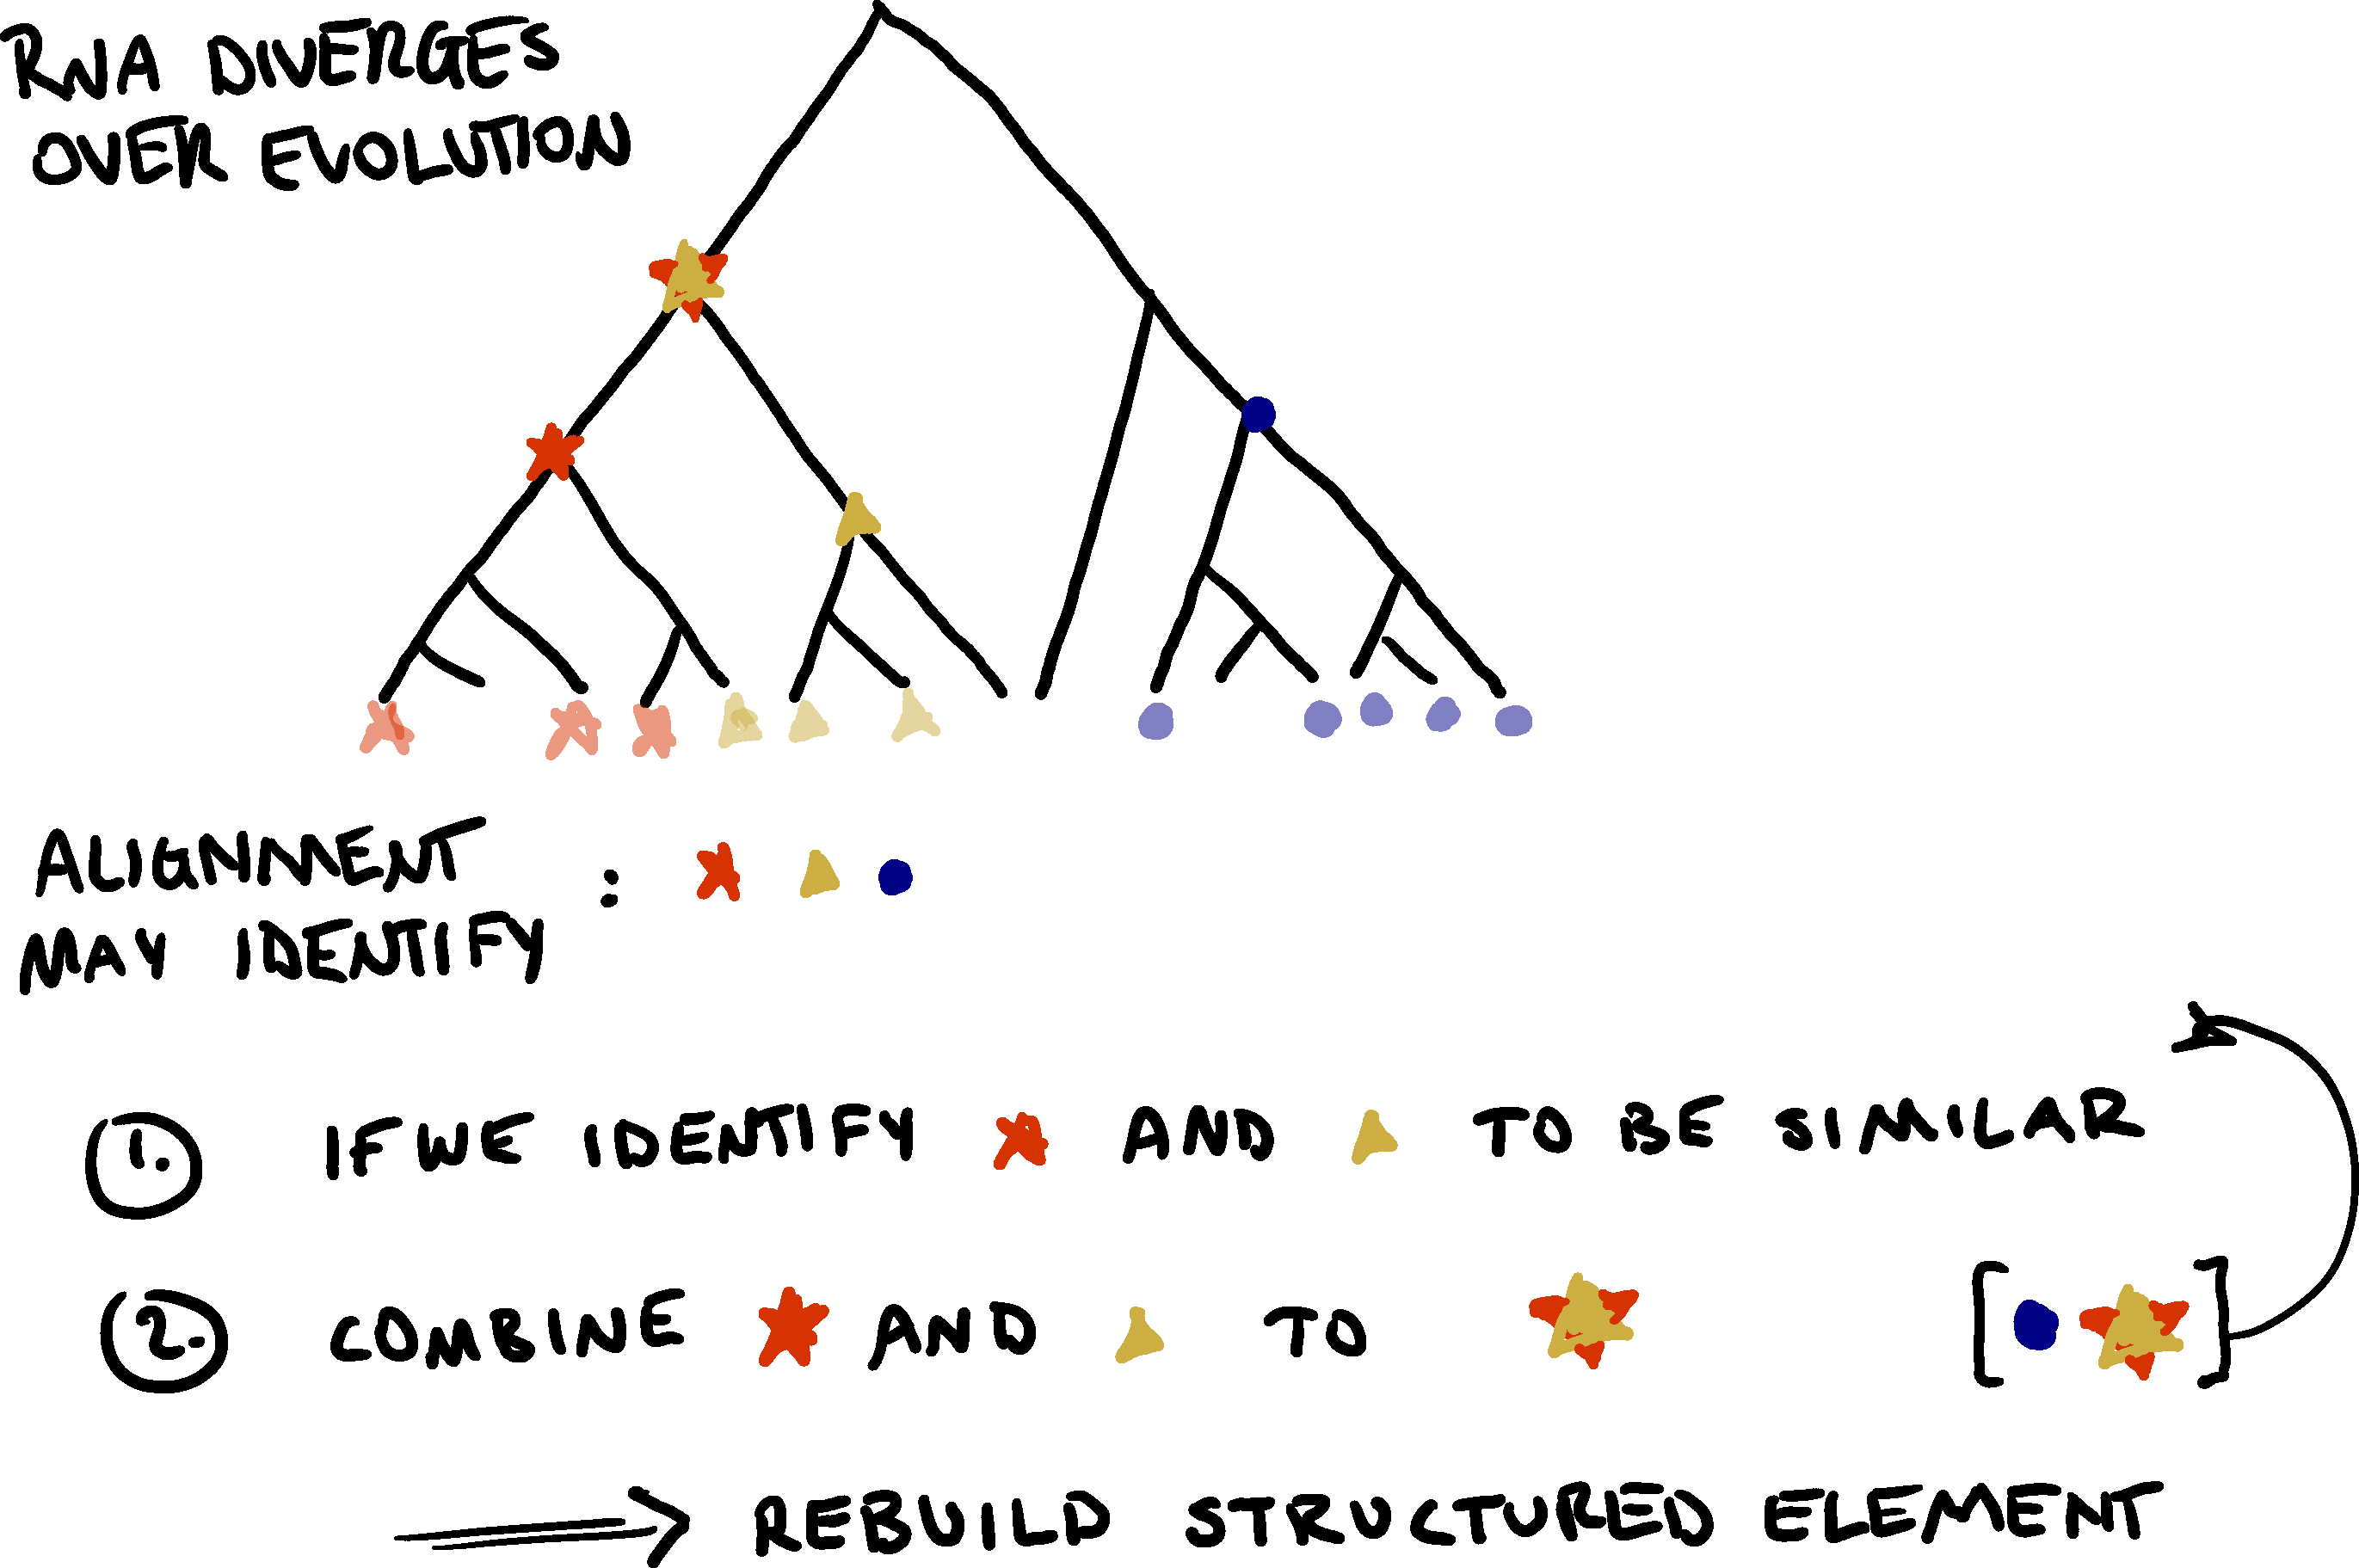
\includegraphics[width=0.8\textwidth]{figures/discussion/cluster-merging.pdf}
    \caption[Covariance model clustering and merging]{\textbf{Covariance model clustering and merging.} 
    Shown in red, gold and blue are structured RNA elements that have been identified by local alignment.
    Identified elements are homologous to each other, but are not similar enough to be detected by classical homology search methods.
    Covariance models describing these elements can be clustered based on their similarity, and merged to create a new model that captures the shared features of the original models. 
    This approach can be used to identify more distant homologs and improve the sensitivity of RNA discovery pipelines.}
    \label{fig:cluster-merging}
\end{figure}

The covariance model combination approach (Figure \ref{fig:cluster-merging}) was attempted in this project, but was not successful.
Implementation was attempted by aligning synthesised sequences from each model and then building a new model from the resulting alignment.
This was either done by aligning the sequences with a multiple sequence alignment tool, or by aligning the models with a covariance model alignment tool.
Testing was done with fractured \ac{FMN} riboswitch models.
The Rfam annotated \ac{FMN} seed sequences (Section~\ref{subsec:covariance-models}) were clustered, aligned, structure predicted and built into covariance models as in the final steps of the computational discovery pipeline (Sections~\ref{subsec:clustering}, \ref{subsec:rna-alignment}, \ref{subsec:covariance-analysis} and \ref{sec:build_cm}).
Models were then clustered and iteratively merged, and the resulting model was tested against the original \ac{FMN} riboswitch model.
Neither alignment method was successful in producing new models which scored well (with the combined \ac{KS} D value) against the original \ac{FMN} riboswitch model.
These results were preliminary and not reported.
Further work is needed to develop a reliable method for combining covariance models, and to test the resulting models against known structured RNA elements.
Also, compared to classical homology search methods, this approach is computationally expensive and time-consuming, and so may not be practical for large-scale RNA discovery pipelines.

\section{Conclusions}

The first aim of this project was to screen for conserved RNA structural elements located near the \ac{BLUF} domain.
This was achieved, and two candidate structured RNA elements were identified.
The candidates had weak covariation signal and low-confidence interaction predictions.
Further work is needed to validate these candidates, and to determine if they are functional RNAs or involved in light sensing.

The second aim was to develop a protein-first structured RNA discovery pipeline.
This was achieved, and the pipeline was tested with a positive control and a negative control set.
The positive control \ac{FMN} riboswitch was successfully recovered.
This showed the feasibility of a protein-first approach to RNA discovery.
The negative control set provided a baseline for the covariation signal expected when no known structured RNA is present.
Most negative control candidates were found to have weak covariation signal.
One candidate (flagellin candidate 327) produced a strong false-positive covariation signal, and was found to be a conserved protein-coding sequence rather than a structured RNA.
The pipeline is reusable and could be used to screen for conserved RNA structural elements associated with other protein domains in future work.

The third aim was to develop a method for clustering covariance models based on their similarity.
This was a later addition to the project, after realising that there was a gap in bioinformatic tools for a fast, working, reliable and statistically defensible similarity scoring.
Several approaches were developed and tested, all capable of clustering Rfam RNA families into their annotated clans (Table~\ref{tab:tab:classifier_comparison}).
Further work is needed to refine this clustering approach and to better validate it.

Overall, the aims of this project were achieved, and a reusable discovery pipeline was developed and tested.
There is some evidence for the use of a protein-first approach to RNA discovery, and the discovery pipeline could be used to screen for conserved RNA structural elements associated with other protein domains in future work.
Beyond this, there is value in finding structured RNA elements and gaining a better understanding of their biological roles, and in developing bioinformatic tools to support this work.

\section{Limitations}

Several limitations apply to the discovery pipeline and the results presented in this project.
The positive control was a single, relatively easy run: the \ac{FMN} riboswitch is highly conserved and well characterised, and the protein domain profile used as the anchor was generated from sequences neighbouring the Rfam-annotated riboswitch.
Recovery of this signal therefore represents a best-case scenario, and is not a general measure of the sensitivity of the pipeline to less conserved or more divergent RNAs.
The negative controls were imperfect, since a domain cannot be proven to lack an associated RNA, only four domains were tested in a single genus, and one of them (flagellin) is itself a less certain negative given reports of RNA regulation of flagellar genes \citet{Mika2013}.
One flagellin candidate scored highly but was protein-coding, so the covariation score alone cannot distinguish a structured RNA from a conserved coding sequence.
Overall, controls were limited, partially by the nature of discovery pipelines, but further work should include a larger set of positive and negative controls, and a more diverse set of protein domains and bacterial species.

The \ac{BLUF} search was restricted to a single genus, \emph{Burkholderia}, and the covariation signal for both \ac{BLUF}-associated candidates was weak.
For each candidate, the original or the iteratively expanded alignment was chosen according to which gave stronger covariation, which adds analytic flexibility.
AlphaFold~3 interface confidence scores (ipTM) were low for both candidates and for the positive control, so the predicted complexes provide no evidence of a specific interaction.
Finally, no experimental validation was performed, so the candidates should be regarded as hypotheses rather than confirmed functional RNAs.

Screening is also limited to just up and down stream of same strand, as we saw with the CRISPR-DR42 conserved RNA protein associations can go beyond this limited relationship.
The discovery pipeline could be extended to mine structured RNAs from more distant intergenic regions, and from the opposite strand to the protein coding gene.
Further, the pipeline currently only searches for structured RNAs associated with a single protein domain, but could be extended to search for structured RNAs associated with multiple protein domains, or with a combination of protein domains and other genomic features.

There are also limitations which arrise from the use of unreliable genome annotations.
The discovery pipeline relies on the accuracy of genome annotations and proteom translations to identify protein coding genes and their associated intergenic regions.
These are known to be error-prone\citep{Salzberg2019}, and despite filtering for contamination and completeness, it is likely that some of the genomes used in this project contain annotation errors.
It is possible these errors play at least some role in the lack of complete consensus on position relative to homologous protein coding gene for the tested riboswitch cases (Table~\ref{tab:results_summary}).

There will also be limitations in the homology searches, both from the protein domain profile searches and from the clustering and alignment steps.
Some of this is unavoidable and a result of the twilight zone of homology, where sequences are too divergent to be detected by homology search methods \citep{Rost1999,McGimpsey2019}.

Overall, there are many limitations to the discovery pipeline and the results presented in this project, but ultimately is intended to be a quick approach to checking for conserved RNA structural elements located near a protein domain of interest.
Once a candidate is identified, further work is needed to validate it and determine if it is a functional RNA or involved in the biological process of interest.

\section{Future directions}

\subsection{Discovery pipeline extension}

There are many ways in which the discovery pipeline could be extended and improved.
These include improving the tool selection, filtering steps and tool parameters for the discovery pipeline, and incorporating additional tools for structural clustering and alignment of RNA elements.
With a wider range of positive and negative controls, the discovery pipeline could be further optimised for speed and sensitivity.
This could introduce some bias in the way current curated RNA elements are identified and lead to overfitting, but would be a useful exercise to improve the discovery pipeline.

The covariance model clustering approach could be integrated into the discovery pipeline to identify similar covariance models and merge them to create a new model that captures the shared features of the original models.
This would allow for the identification of more distant homologs and improve the sensitivity of RNA discovery pipelines, and power of any covariance analysis.
The alignment and covariance analysis steps would not need to identify deep homology or strong covariation signal, as the clustering and merging of covariance models would allow for the identification of more distant homologs.

There may be other tools that could be used to improve the discovery pipeline, and the pipeline could be further optimised for speed and sensitivity.
A preprint from September 2026, \citet{Li2026}, describes a new approach to the discovery of RNA protein systems, using a large language model to identify non-coding elements coevolving with proteins.
Their apprach predicts pairwise interactions between nucleotides and proteins, and has had success with identifying known structured RNA elements and their associated proteins.
This approach could be used to identify targets for \ac{RNP} discovery, or this idea of coevolution could be incorporated into the discovery pipeline to improve the likelihood of finding functional \ac{RNP} systems.
Another tool, RNA-align \citep{Gong2019}, aligns RNA secondary structures and could be used to improve the clustering of candidate RNA elements.
\citet{McGimpsey2019} describe an iterative approach to homology search using nhmmer, which they found to lower the twilight zone of RNA homology.
This approach could be used to improve the sensitivity of the nucleotide homology searches in the discovery pipeline, and a similar approach could be taken for the protein domain profile searches.
Further works should explore the use of these tools in the discovery pipeline, and compare their performance to the current approach.

Further binary logic could be added to the discovery pipeline to filter candidates based on their genomic context, such as their proximity to other genes or regulatory elements.
For example, non coding regions that are located near one light related protein domain or another light related protein domain, or one pathway related protein and a different pathway related protein.
This could be used to identify candidates in a more complex biology aware manner.

\subsection{Further targets for \ac{RNP} discovery}

There are endless possibilities for further targets for \ac{RNP} discovery, and the discovery pipeline could be applied to a wide range of protein domains and biological processes.
Expand beyond \ac{BLUF}, other light-pathway anchors (e.g. phytochromes, cryptochromes) and other photoreceptor families could be used to anchor searches for further \ac{RNP} or cis-regulatory candidates.
These searches could be extended to other bacterial species, and to other kingdoms of life, including archaea and eukaryotes.

With the success of \citet{Durrant2024} in identifying the novel Bridge RNA recombinase system, TIGR from \citet{Bruck2025}, and the earlier discovery of \ac{CRISPR} \citep{Barrangou2007}, it would be interesting to apply the discovery pipeline to other DNA editing proteins.
\ac{RNP} complex discoveries like this have the potential to be significant biotechnological tools, as the previous examples highlight.

\subsection{Experimental validation}

Once a candidate structured RNA element is identified, and further investigated by computational methods, it should be experimentally validated.
Neither of the \ac{BLUF}-associated candidates identified in this project are currently particularly convincing as structured RNA elements, but if further work found more evidence for them, or if other candidates were identified, they should be experimentally validated.
Chemical probing methods, such as \ac{SHAPE-seq} \citep{Lucks2011} or \ac{DMS-MaPseq} \citep{Zubradt2017}, could be used to determine the secondary structure of the RNA element.
Also, depending on the predicted function of the RNA element, experimental assays could be used to determine its biological role, such as real time quantitative \ac{PCR} and stimulus-response experiments for cis-regulatory elements.